\section{Podobné aplikácie}
\subsection{Mapbox}
Mapbox je platforma údajov o polohe pre mobilné a webové aplikácie\cite{mapbox}. Poskytuje mnoho produktov: \textit{Mapbox GL JS} knižnicu, pomocou ktorej je možné vytvoriť interaktívnu, prispôsobenú a efektívnu mapu vo webovej aplikácii\cite{mapbox_gljs}, \textit{Navigation SDK for mobiles}, riešenie pre vytváranie navigácie v mobilných telefónoch dostupné pre \textit{Android} aj \textit{iOS}\cite{mapbox_mobile_navigation},  \textit{MapGPT}, prvého \acrshort{ai} asistenta, s ktorým je možné mať konverzácie ohľadom ciest, navigačných inštrukcií alebo atrakcií\cite{mapbox_mapgpt}. Výhody Mapboxu:
\begin{itemize}
    \item Ponúka 50 tisíc načítaní mapy vo webovej aplikácii.
    \item Poskytuje map-matching, ktorý pripne vstupné GPS údaje trasy k cestnej sieti pre zaručenie prehľadného zobrazenie trás, to znamená, že trasy nebudú zobrazené mimo cesty ale budú ležať na cestnej sieti.
    \item Prispôsobenie štýlov mapy, markerov alebo vyskakovacích okien.
\end{itemize}
Nevýhody
\begin{itemize}
    \item Neposkytuje vlastnú webovú aplikáciu, na ktorú je možné nahrať trasu, ktorú chceme zobraziť. Trasa sa dá zobraziť až po použití Mapbox GL JS a implementovaní vlastnej webovej aplikácie.
    \item Vstupné dáta treba upraviť na požadovaný formát pred odoslaním do Mapbox \acrshort{api}.
    \item Do jednej požiadavky na map-match je možné vložiť len 100 bodov, preto je potrebné pre dlhšie trasy (tisíc bodov a viac) urobiť niekoľko požiadaviek. Pri aplikácií, ktorú používa veľa používateľov (rádovo tisíc) môže rýchlo dôjsť k vyčerpaniu kvóty pre map-match (100 tisíc mesačne) zadarmo. Taktiež rozdelenie trás do viacerých požiadaviek spomaľuje rýchlosť map-matchingu.
    \item Trasa je ku cestnej sieti pripnutá nepresne, viď obrázok \ref{fig:mapbox-map-match-vs-valhalla}.
    \item Je potrebné použiť online \acrshort{api}, čo môže spomaliť map-matching.
\end{itemize}

\begin{figure}[H]
\centering
\begin{subfigure}{.45\textwidth}
  \centering
  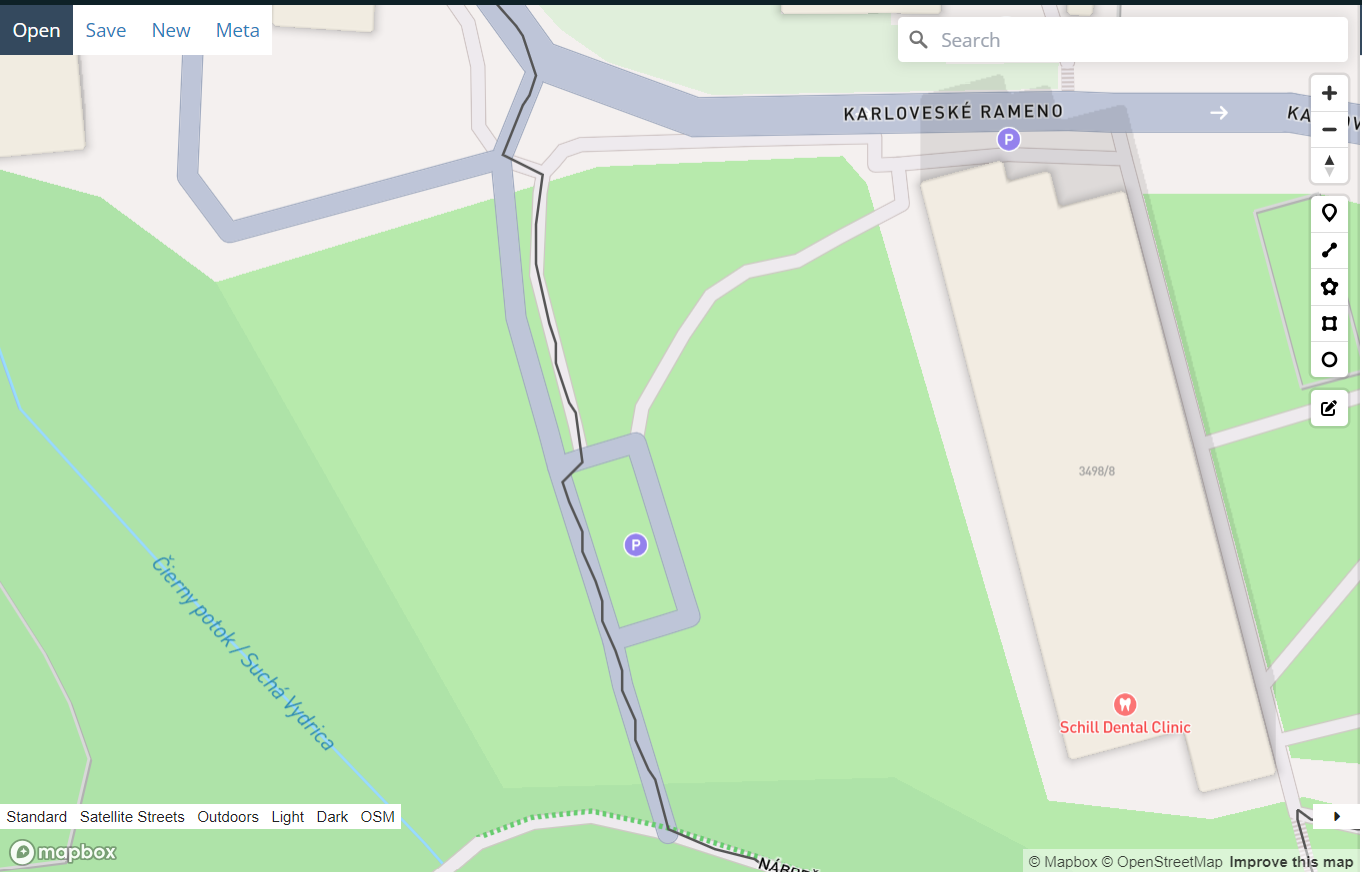
\includegraphics[width=1\textwidth]{img/porovnanie_map_match/mapbox-map-match.png}
  \caption{Map-match od Mapbox}
  \label{fig:mapbox-map-match}
\end{subfigure}
\begin{subfigure}{.45\textwidth}
  \centering
  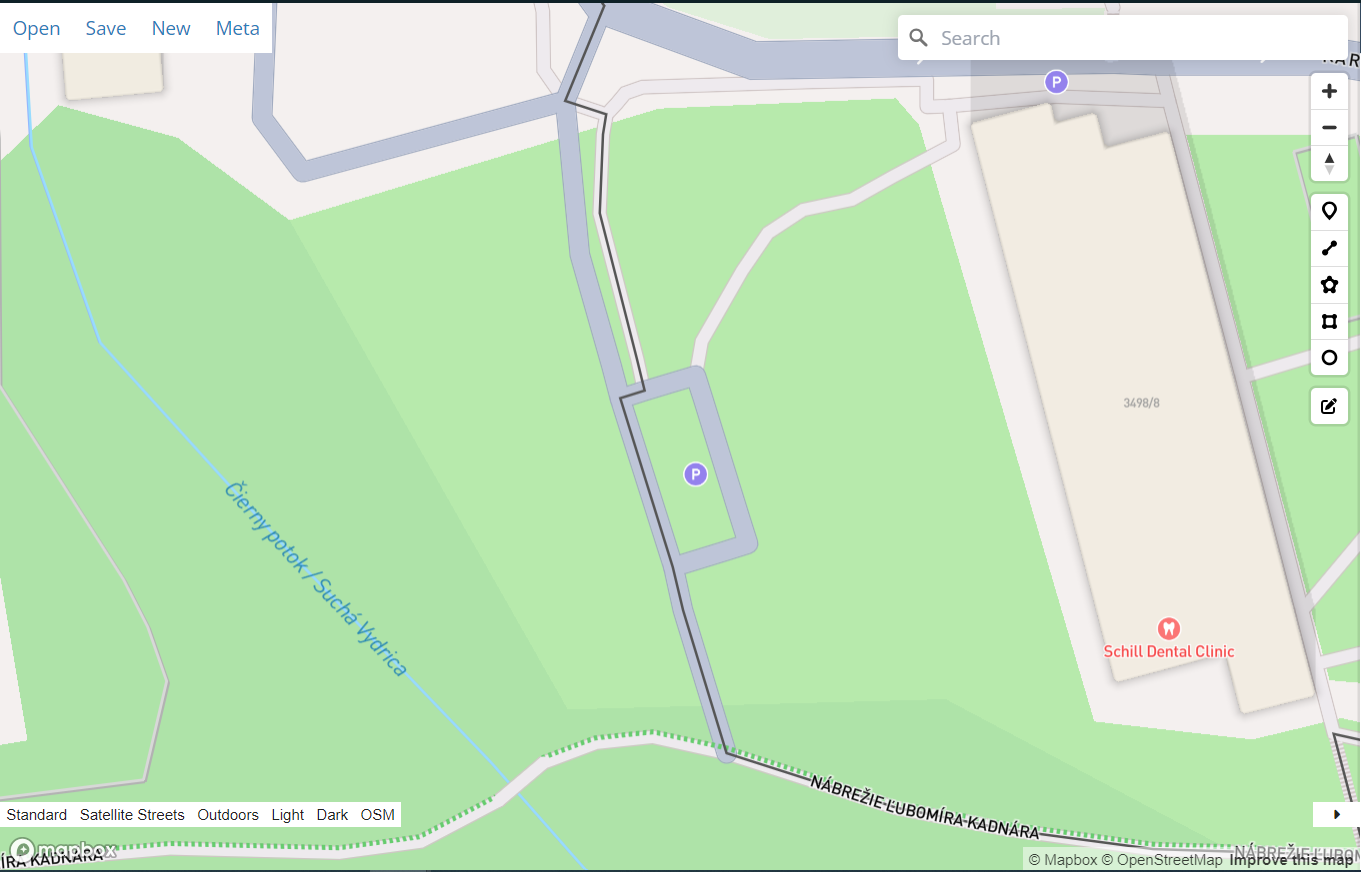
\includegraphics[width=1\textwidth]{img/porovnanie_map_match/valhalla-map-match.png}
  \caption{Map-match od Valhally}
  \label{fig:valhalla-map-match}
\end{subfigure}
\caption{Porovnanie Mapbox a Valhalla map-matching}
\label{fig:mapbox-map-match-vs-valhalla}
\end{figure}